\chapter{System Overview}

The goal of the system is to classify panorama images into defined classes.
For that a CLIP like network is used on the edge.
As a computing platform a Raspberry Pi 5 with the hardware accelerator extension is used.
The hardware Accelerator is the Hailo-8L entry level accelerator (\cref{fig:overview:aikit}).
The System which is used and developt in this work, can be divided in 2 parts.
One part is the compilation of a neural network on a PC.
The other part is the inference of a compiled network on the Raspberry Pi.

\begin{figure}[h]
    \centering
    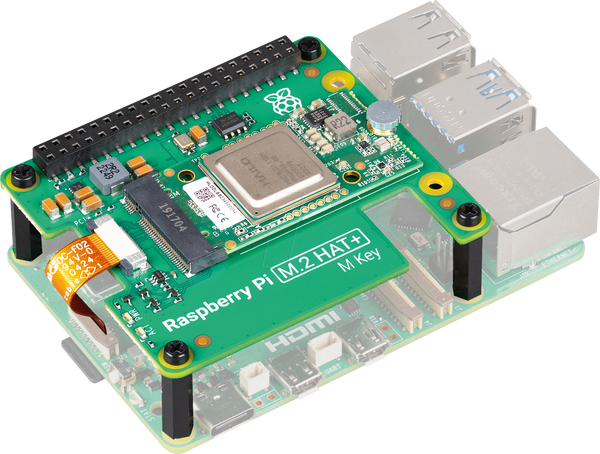
\includegraphics[width=0.5\textwidth]{Images/SystemOverview/ai-kit.png}
    \caption{Picture of the hardware accelerator mounted on a Raspberry Pi 5\cite{bildAiKit}}
    \label{fig:overview:aikit}
\end{figure}



\section{Compilation of a Network}

\begin{figure}
    \centering
    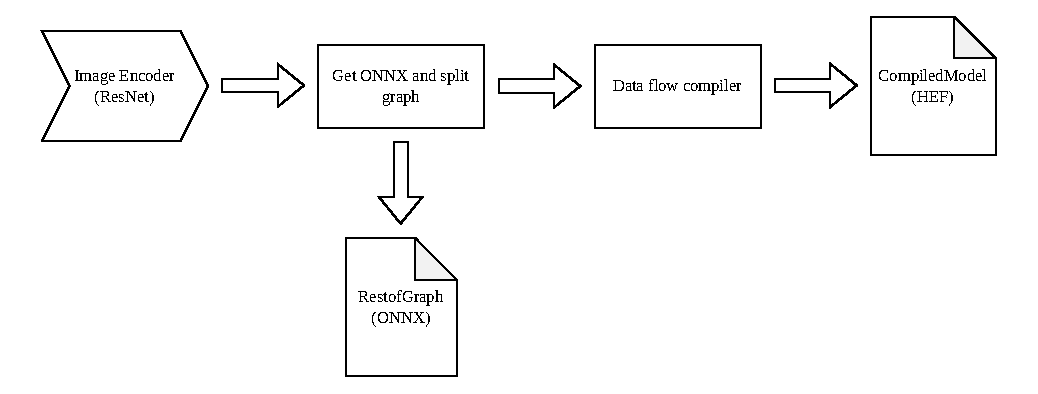
\includegraphics[width=\textwidth]{Images/SystemOverview/DFCFlow.pdf}
    \caption{Visualisation of the compilation work flow}
    \label{fig:overview:dfcflow}
\end{figure}
First the image encoder either from \acrshort{clip} or TinyCLIP has to be aquuired.
This encoder then gets exported as a ONNX graph.
The part from the graph which doesn't compile gets cut of and saved for later.
Then the edited graph gets compiled.
During compilation, the network is quantized and simplified.
This reduces the amount of memory and processing power needed to use a network.
The network has to be compiled to format which can be executed on the hardware accelerator.
In this work the compilation is done with the \Acrlong{dfc} (see \cref{section:dfc}) from Hailo.
The result is a \acrshort{hef} file which can be executed on hailo hardware.

\section{Inference on Raspberry Pi}

\begin{figure}
    \centering
    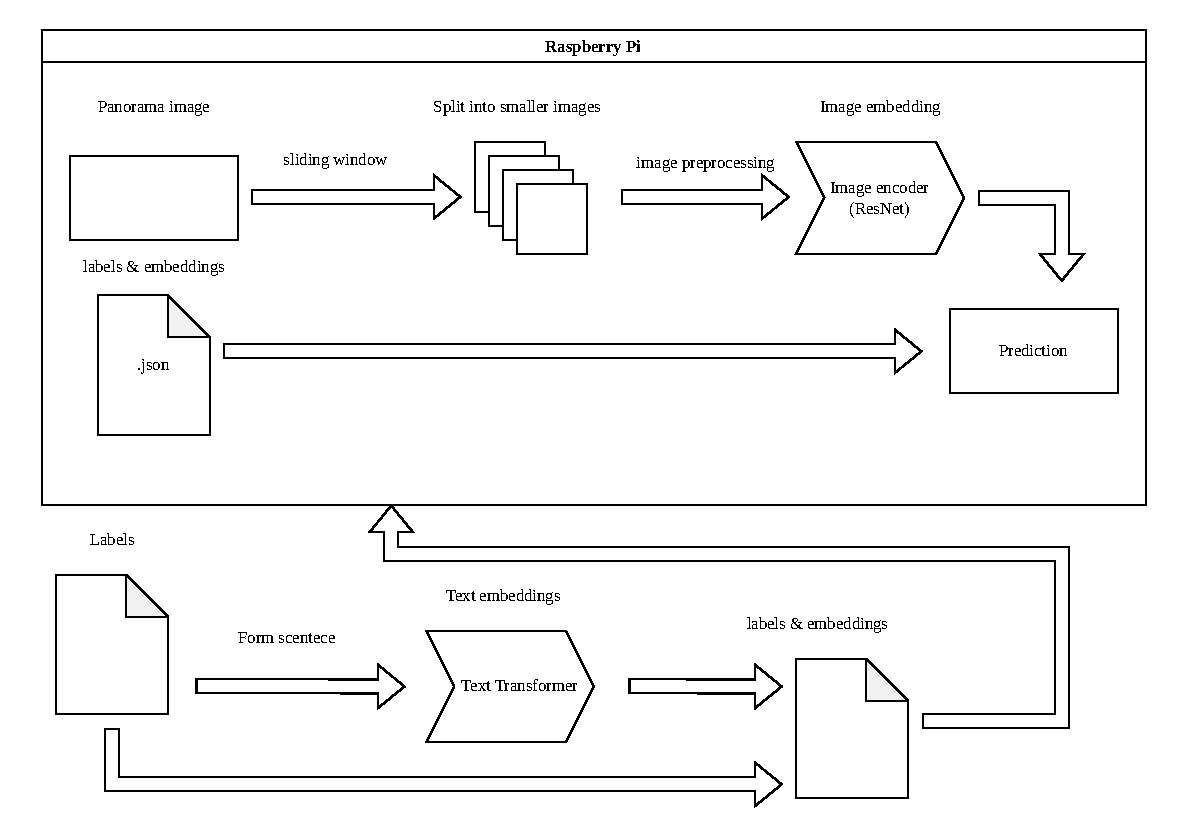
\includegraphics[width=\textwidth]{Images/SystemOverview/Overview.drawio.pdf}
    \caption{System work flow}
    \label{fig:overview:overview}
\end{figure}

To use a network on a hardware accelerator a specific software has to be used.
Because of current limitations of the \acrshort{dfc}, self attention layers were unable to compile.
Because of this constraint the text encoder of CLIP must be executed in advance on an PC.
The resulting text embeddings then get loaded on to the Raspberry Pi in form of a json file.
The text embedding consist of the expressions from \cref{tab:dataset:subclasses} subclasses.
These expressions are wrapped in 5 scentens to further increase accuracy.
The constrain also doesnt allow transformers to compile.
Because of that reason ResNets were used as image encoders.
The problem with the resnets was, that the last layer also is a self attention layer.
To get the network to compile, the last part got cut off and is later processed as a from of postprocessing.
The panorama pictures are split up into 5 pictures which are classified sepertatly.
To get the final prediction a mayority vote over the 5 image patches gets taken.

